\documentclass[12pt]{article}
\usepackage{amsmath}
\usepackage{amsthm}
\usepackage{amssymb}
\usepackage{euscript}
\usepackage{mathrsfs}
\usepackage{bm}
\usepackage{enumitem}
\usepackage{tikz}
\usepackage{mathtools}
\usepackage{float}
\usepackage{hyperref}
\usepackage{boldline}
\usepackage{indentfirst}
\usepackage{environ}
\usepackage{courier}
\usetikzlibrary{positioning}

\renewcommand{\labelitemii}{$\vartriangleright$}
\renewcommand{\labelitemiv}{$\Join$}

\makeatletter
\newsavebox{\measure@tikzpicture}
\NewEnviron{scaletikzpicturetowidth}[1]{%
  \def\tikz@width{#1}%
  \def\tikzscale{1}\begin{lrbox}{\measure@tikzpicture}%
  \BODY
  \end{lrbox}%
  \pgfmathparse{#1/\wd\measure@tikzpicture}%
  \edef\tikzscale{\pgfmathresult}%
  \BODY
}
\makeatother

\numberwithin{equation}{section}

\hypersetup{
    colorlinks=true,
    % linkcolor=blue,
    linkcolor=[RGB]{0,0,128},
    % filecolor=[RGB]{0,0,128},
    filecolor=magenta,
    urlcolor=cyan,
    citecolor = [RGB]{128,0,128}
}

\newcommand{\myref}[2]{\hyperref[#2]{#1 \ref*{#2}}}
\newcommand{\myrefT}[1]{\hyperref[#1]{Theorem \ref*{#1}}}
\newcommand{\myrefP}[1]{\hyperref[#1]{Proposition \ref*{#1}}}
\newcommand{\myrefL}[1]{\hyperref[#1]{Lemma \ref*{#1}}}
\newcommand{\myrefD}[1]{\hyperref[#1]{Definition \ref*{#1}}}
\newcommand{\myrefn}[3]{\hyperref[#2]{#1 \ref*{#2} (#3)}}

% \input{dynkinMacros.tex}
% \input{dynkinEMacros.tex}
% \renewcommand{\qedsymbol}{}
\newcommand{\ssm}{\smallsetminus}

\newcommand{\para}[1]{\noindent\underline{#1}.}

\newcommand{\ti}{$\tau\textnormal{-invariant}$}
\newcommand{\prim}{\textnormal{Prim}_{\lambda}(\textnormal{U}(\gf))}

\newcommand{\ve}{\varepsilon}
\newcommand{\veo}{\varepsilon_1}
\newcommand{\vet}{\varepsilon_2}
\newcommand{\vei}{\varepsilon_i}
\newcommand{\vp}{\varphi}

% \newcommand{\inr}{\textnormal{In}^R}
% \newcommand{\inl}{\textnormal{In}^L}
% \newcommand{\inc}{\textnormal{In}}
% \renewcommand{\sc}{\textnormal{SC}}
% \newcommand{\re}{\textnormal{Re}}

\newcommand{\ag}{\alpha}
\newcommand{\bg}{\beta}
\newcommand{\g}{\gamma}
\newcommand{\dg}{\delta}
\newcommand{\rg}{\rho}
\newcommand{\kg}{\kappa}
\newcommand{\sg}{\sigma}
\newcommand{\tg}{\tau}
\renewcommand{\lg}{\lambda}

\renewcommand{\gg}{$\gamma \ $}
\newcommand{\ga}{$\alpha \ $}
\newcommand{\gt}{$\tau $}
\renewcommand{\(}{(\gamma)}
\newcommand{\atg}{\tilde\alpha}
\newcommand{\ags}[1]{{\ag_{#1}}}
\newcommand{\ao}{{\ag_1'}}

\newcommand{\gf}{\mathfrak g}
\newcommand{\hf}{\mathfrak h}

% needs a new name
%\newcommand{\th}[1]{{$\text{\it #1 }^{\underline{\textnormal{th}}}$}}
\renewcommand{\sf}{\mathscr F}
\newcommand{\dsf}{$\sf$}
\newcommand{\st}{\mathscr T}
% needs a new name  -- ok?
\newcommand{\so}[1]{\mathscr #1}


\newcommand{\snn}{{\mathscr S(n,n)}}
\newcommand{\smm}{{\mathscr S(M^L,M^R)}}
\renewcommand{\tan}{\mathscr T_A(n)}
\newcommand{\tn}{\mathscr T(n)}
\newcommand{\dtn}{$\tn$}
\newcommand{\tm}{\mathscr T(M)}
\newcommand{\dtm}{$\tm$}
\newcommand{\tcsn}{\mathscr T_C^S(n)}
\newcommand{\tbsn}{\mathscr T_B^S(n)}
\newcommand{\tsn}[1]{\mathscr T_#1(n)}
\newcommand{\tsm}[1]{\mathscr T_#1(M)}
\newcommand{\tnn}{\mathscr T(n,n)}
\newcommand{\tmm}{\mathscr T(M^L,M^R)}
\newcommand{\tkmm}{\mathscr T_K(M^L,M^R)}
\newcommand{\tsnn}[1]{\mathscr T_#1(n,n)}
\newcommand{\tsmm}[1]{\mathscr T_#1(M^L,M^R)}
\newcommand{\tdnn}{\mathscr T_D(n,n)}
\newcommand{\tdmm}{\mathscr T_D(M^L,M^R)}
\newcommand{\tdn}{\mathscr T_D(n)}
\newcommand{\tdm}{\mathscr T_D(M)}
\newcommand{\tcnn}{\mathscr T_C(n,n)}
\newcommand{\tcmm}{\mathscr T_C(M^L,M^R)}
\newcommand{\tcn}{\mathscr T_C(n)}
\newcommand{\tcm}{\mathscr T_C(M)}
\newcommand{\cm}{\mathscr C(M)}
\newcommand{\dm}{\mathscr D(M)}

\newcommand{\snnp}{\mathscr S'(n,n)}
\newcommand{\smmp}{\mathscr S'(M^L,M^R)}
\newcommand{\snnpp}{\mathscr S''(n,n)}
\newcommand{\smmpp}{\mathscr S''(M^L,M^R)}
\newcommand{\tnnp}{\mathscr T'(n,n)}
\newcommand{\tmmp}{\mathscr T'(M^L,M^R)}
\newcommand{\tnnpp}{\mathscr T''(n,n)}
\newcommand{\tmmpp}{\mathscr T''(M^L,M^R)}
\newcommand{\tdnnp}{\mathscr T_D'(n,n)}
\newcommand{\tdmmp}{\mathscr T_D'(M^L,M^R)}
\newcommand{\tdnnpp}{\mathscr T_D''(n,n)}
\newcommand{\tdmmpp}{\mathscr T_D''(M^L,M^R)}


\newcommand{\talb}{T_{\alpha \beta}}
\newcommand{\tai}{T_{\alpha_i,\alpha_{i+1}}}
\newcommand{\tap}{T_{\alpha_{i+1},\alpha_i}}
\newcommand{\tao}{T_{\alpha_1,\alpha_2}}
\newcommand{\tat}{T_{\alpha_2,\alpha_1}}

% new
\newcommand{\talbLeft}{T^L_{\alpha \beta}}
\newcommand{\talbRight}{T^R_{\alpha \beta}}

\newcommand{\ot}{\overline T}
\newcommand{\og}{\overline{\gamma}}

\newcommand{\sij}{{S_{ij}}}
\renewcommand{\ss}[2]{{S_{#1,#2}}}
% \def\ss#1#2{S_{#1,#2}}

\newcommand{\im}{{i-1}}
% \renewcommand{\ip}{{i+1}}
\newcommand{\ip}{{i+1}}
\newcommand{\imm}{{i-2}}
\newcommand{\ipp}{{i+2}}
\newcommand{\jm}{{j-1}}
\newcommand{\jp}{{j+1}}
\newcommand{\jmm}{{j-2}}
\newcommand{\jpp}{{j+2}}

\renewcommand{\tt}{\tau (T)}
\newcommand{\abe}{{$\{\ag,\bg\}=\{\ag_i,\ag_\ip\}$}}

\newcommand{\bt}{\mathbf T}
\newcommand{\bto}{\mathbf T_1}
\newcommand{\btt}{\mathbf T_2}
\newcommand{\obt}{\overline\bt}
\newcommand{\obto}{\overline\bt_1}
\newcommand{\obtt}{\overline\bt_2}
\newcommand{\tbt}{\tilde\bt}
\newcommand{\tbto}{\tilde\bto}
\newcommand{\tbtt}{\tilde\btt}
\newcommand{\pbt}{(\bto,\btt)}
\newcommand{\pbtp}{(\bto',\btt')}
\newcommand{\pobt}{(\obto,\obtt)}
\newcommand{\pbts}[1]{(\bto^{#1},\btt^{#1})}
\newcommand{\pobts}[1]{(\obto^{#1},\obtt^{#1})}
\newcommand{\pobtp}{(\obto',\obtt')}

\newcommand{\lo}{(\bto,\bt)}
\newcommand{\lop}{(\bto',\bt)}
\newcommand{\ls}[1]{(\bt_#1,\bt)}
\newcommand{\lsp}[1]{(\bt_#1',\bt)}
\newcommand{\ol}{(\obt_1,\obt)}

\newcommand{\be}{\mathbf E}
\newcommand{\bs}{\mathbf S}
\newcommand{\bl}{\mathbf L}
\newcommand{\br}{\mathbf R}
% \renewcommand{\op}{\bar P}
\newcommand{\op}{\bar P}
\newcommand{\pe}{P_e}

\newcommand{\oc}{\overline c}
\newcommand{\cL}{\prescript{L}{}{c}}
\newcommand{\cR}{\prescript{R}{}{c}}
\newcommand{\bc}{\mathbf c}
\newcommand{\bcL}{\prescript{L}{}{\bc}}
\newcommand{\bcR}{\prescript{R}{}{\bc}}
\newcommand{\overbc}{\overline{\mathbf c}}
\newcommand{\overcL}{\prescript{L}{}{\overline c}}
\newcommand{\overcR}{\prescript{R}{}{\overline c}}
\newcommand{\overbcL}{\prescript{L}{}{\overbc}}
\newcommand{\overbcR}{\prescript{R}{}{\overbc}}

% \newcommand{\sha}{{\textnormal{Shape}}}
\newcommand{\cs}{{c.s.p.b.}}
% \newcommand{\OC}{{\textnormal{OC}}}
% \newcommand{\OCS}{{\textnormal{OC*}}}
\newcommand{\Sf}{S_f}
\newcommand{\Sb}{S_b}
\newcommand{\nh}{n_h}
\newcommand{\nv}{n_v}
\newcommand{\rinf}{\rg_{\inf}}
\newcommand{\rsup}{\rg_{\sup}}

\newcommand{\ec}{\underset {ec}\sim}
\newcommand{\gtl}{\underset {GTL}\sim}
\newcommand{\en}{\underset {n}\sim}
\newcommand{\enm}{\underset {n-1}\sim}
\newcommand{\eqm}{\underset {m}\sim}
\newcommand{\eqmm}{\underset {m-1}\sim}
\newcommand{\ez}{\underset {0}\sim}
\newcommand{\gtr}{\underset {GTR}\sim}
\renewcommand{\gt}{\underset {GT}\sim}
\newcommand{\ngtl}{\underset {GTL}\nsim}
\newcommand{\jl}{\underset {JL}\sim}
\newcommand{\jr}{\underset {JR}\sim}
\newcommand{\kll}{\underset {KLL}\sim}
\newcommand{\klr}{\underset {KLR}\sim}

\newcommand{\fo}{F_1}
\newcommand{\ft}{F_2}
\newcommand{\fot}{\tilde\fo}
\newcommand{\ftt}{\tilde\ft}

\newcommand{\bi}{{\it b}){\it i})}
\newcommand{\bii}{{\it b}){\it ii})}

\newcommand{\sig}{\Sigma}
\newcommand{\tsl}{T_\Sigma^L}
\newcommand{\tspl}{T_{\Sigma'}^L}
\newcommand{\tssl}[1]{T_{\Sigma^#1}^L}
\newcommand{\tssbl}[1]{T_{\Sigma_#1}^L}
\newcommand{\ts}{T_\Sigma}
\newcommand{\tsp}{T_{\Sigma'}}
\newcommand{\tss}[1]{T_{\Sigma^#1}}
\newcommand{\tssb}[1]{T_{\Sigma_#1}}
\newcommand{\pin}{$\Pi\ssm\{\ag_n\}$}
\newcommand{\pc}{\phi_C}
% \newcommand{\pd}{{\phi_D}}
\newcommand{\il}{I_\lg}

\newcommand{\te}[1]{\textnormal{#1}}

\newcommand{\plainTL}{\prescript{L}{}{T}}
\newcommand{\plainTR}{\prescript{R}{}{T}}

\newcommand{\tL}{\prescript{L}{}{\bt}}
\newcommand{\tR}{\prescript{R}{}{\bt}}
\newcommand{\pairTLR}{(\tL,\tR)}
\newcommand{\pairTLRPrime}{(\tL',\tR')}
\newcommand{\pairTLRSub}[1]{(\tL_{#1},\tR_{#1})}
\newcommand{\pairTLRPrimeSub}[1]{(\tL'_{#1},\tR'_{#1})}

\newcommand{\overTL}{\prescript{L}{}{\obt}}
\newcommand{\overTR}{\prescript{R}{}{\obt}}
\newcommand{\overPairTLR}{(\overTL,\overTR)}
\newcommand{\overPairTLRPrime}{(\overTL',\overTR')}
\newcommand{\overPairTLRSub}[1]{(\overTL_{#1},\overTR_{#1})}
\newcommand{\overPairTLRPrimeSub}[1]{(\overTL'_{#1},\overTR'_{#1})}

\newcommand{\tildeTL}{\prescript{L}{}{\tbt}}
\newcommand{\tildeTR}{\prescript{R}{}{\tbt}}
\newcommand{\tildePairTLR}{(\tildeTL, \tildeTR)}
\newcommand{\pairTLRStar}{(\tL^*, \tR^*)}
\newcommand{\overPairTLRStar}{(\overTL^*, \overTR^*)}

\newcommand{\pisn}{{$\Pi^*\ssm\{\ag_n\}$}}

\newcommand{\tLSigma}{\tsl}
\newcommand{\tLSigmaSub}[1]{\tssbl#1}
\newcommand{\tDMM}{\tdmm}

\newcommand{\leftPrime}{(\tL',\tR)}
\newcommand{\leftSub}[1]{(\tL_{#1},\tR)}
\newcommand{\leftPrimeSub}[1]{(\tL_{#1}',\tR)}


\DeclareMathOperator{\Shape}{Shape}
\DeclareMathOperator{\OC}{OC}
\DeclareMathOperator{\OCS}{OC*}
% \newcommand{\inr}{\textnormal{In}^R}
% \newcommand{\inl}{\textnormal{In}^L}
% \newcommand{\inc}{\textnormal{In}}
% \renewcommand{\sc}{\textnormal{SC}}
\newcommand{\re}{\textnormal{Re}}
\DeclareMathOperator{\In}{In}
\newcommand{\inc}{\In}
\newcommand{\inL}{\In^L}
\newcommand{\inR}{\In^R}
\DeclareMathOperator{\SC}{SC}
\newcommand{\scL}{\SC^L}
\newcommand{\scR}{\SC^R}

\DeclareMathOperator{\Adj}{Adj}
\newcommand{\oeta}{\overline{\eta}}

\newcommand{\preL}[1]{\prescript{L}{}{#1}}

\newcommand{\makeBox}[2] {
  \newsavebox{#1}
  \begin{lrbox}{#1}{#2}\end{lrbox}
}

\tikzstyle{tableau} = [y = -1cm, every node/.style={transform shape}]

\definecolor{gridColor}{RGB}{19,83,150}
\tikzstyle{dominoStyle} = [color=black, fill=white, rounded corners = .1cm, thick]
\tikzstyle{gridLine} = [color=gridColor, thick]
\tikzstyle{dominoText} = [font=\Large, midway]
\tikzstyle{cycleLine} = [color=green, thick, >->]
\tikzstyle{closedCycleLine} = [color=green, thick]
% \tikzstyle{fixedSquareStyle} = [pattern = crosshatch doats, pattern color=gridColor,  opacity=0.2]
\tikzstyle{fixedSquareStyle} = [color=gridColor,  opacity=0.07]
\tikzstyle{tileText} = [font=\large, midway]

\newcommand{\eps}{.06}
\newcommand{\teps}{\eps * 2}

% first entry is row, starting with 1, second entry is column, third is content
\newcommand{\filledSquare}[3]{\filldraw [dominoStyle] (#2 - 1 + \eps, #1 - 1 + \eps) rectangle + (1 - \teps, 1 -\teps) node [tileText] {$#3$};}
% The fourth entry shifts vertically
\newcommand{\filledSquareShift}[4]{\filldraw [dominoStyle] (#2 - 1 + #4 + \eps, #1 - 1 + \eps) rectangle + (1 - \teps, 1 -\teps) node [tileText] {$#3$};}

\newcommand{\horizontalDomino}[3]{\filldraw [dominoStyle] (#2 - 1 + \eps, #1 - 1 + \eps) rectangle + (2 - \teps, 1 -\teps) node [dominoText] {$#3$};}
\newcommand{\verticalDomino}[3]{\filldraw [dominoStyle] (#2 - 1 + \eps,  #1 - 1 + \eps) rectangle + (1 - \teps,2 -\teps) node [dominoText] {$#3$};}

\newcommand{\horizontalDominoShift}[4]{\filldraw [dominoStyle] (#2 - 1 + #4 + \eps, #1 - 1 + \eps) rectangle + (2 - \teps, 1 -\teps) node [dominoText] {$#3$};}
\newcommand{\verticalDominoShift}[4]{\filldraw [dominoStyle] (#2 - 1 + #4 + \eps,  #1 - 1 + \eps) rectangle + (1 - \teps,2 -\teps) node [dominoText] {$#3$};}

\newcommand{\zeroSquare}[2]{\filldraw [dominoStyle] (#2 - 1 + \eps, #1 - 1 + \eps) rectangle + (1 - \teps, 1 -\teps) node [dominoText] {$0$};}
\newcommand{\zeroSquareShift}[3]{\filldraw [dominoStyle] (#2 - 1 + #3 + \eps, #1 - 1 + \eps) rectangle + (1 - \teps, 1 -\teps) node [dominoText] {$0$};}


\newcommand{\emptyBox}[2]{\filldraw [dominoStyle] (#2 - 1 + \eps, #1 - 1 + \eps) rectangle + (2 - \teps, 2 -\teps);}
\newcommand{\signedBox}[3]{
\filldraw [opacity=0] (#2 - 1 + 1, #1 - 1) rectangle + (1, 2) node [dominoText,opacity=1] {$#3$};
\filldraw [dominoStyle, fill opacity = 0] (#2 - 1 + \eps, #1 - 1 + \eps) rectangle + (2 - \teps, 2 -\teps);
}

\newcommand{\emptyBoxShift}[3]{\filldraw [dominoStyle] (#2 - 1 + #3 + \eps, #1 - 1 + \eps) rectangle + (2 - \teps, 2 -\teps);}
\newcommand{\signedBoxShift}[4]{
\filldraw [opacity=0] (#2 - 1 + 1 + #4, #1 - 1) rectangle + (1, 2) node [dominoText,opacity=1] {$#3$};
\filldraw [dominoStyle, fill opacity = 0] (#2 - 1 + #4 + \eps, #1 - 1 + \eps) rectangle + (2 - \teps, 2 -\teps);
}

% These rows and columns are zero-based
\newcommand{\horizontalGridLine}[3]{\draw [gridLine] (#1, #2) -- + (#3,0);}
\newcommand{\verticalGridLine}[2]{\draw [gridLine] (#1, 0) -- + (0,#2);}
\newcommand{\fixedSquare}[2]{\filldraw [fixedSquareStyle] (#1,#2) rectangle +(1,1);}

% This will have #1 * 2 rows and #2 *2 columns
\newcommand{\gridLines}[2] {
  \pgfmathsetmacro{\verticalEnd}{2 * #1}
  \pgfmathsetmacro{\horizontalEnd}{2 * #2}
  \foreach \vertical in {0,...,#2} {
    \pgfmathsetmacro{\var} {2 * \vertical}
    \verticalGridLine{\var}{\verticalEnd}
  }
  \foreach \horizontal in {0,...,#1} {
    \pgfmathsetmacro{\var} {2 * \horizontal}
    \horizontalGridLine{0}{\var}{\horizontalEnd}
  }
}

% This will have #1 * 2 rows and #2 *2 columns
% The vertical lines will be shifted over #3 squares
\newcommand{\gridLinesShift}[3] {
  \pgfmathsetmacro{\verticalEnd}{2 * #1}
  \pgfmathsetmacro{\horizontalEnd}{2 * #2}
  \foreach \vertical in {0,...,#2} {
    \pgfmathsetmacro{\var} {2 * \vertical + #3}
    \verticalGridLine{\var}{\verticalEnd}
  }
  \foreach \horizontal in {0,...,#1} {
    \pgfmathsetmacro{\var} {2 * \horizontal}
    \horizontalGridLine{#3}{\var}{\horizontalEnd}
  }
}

\newcommand{\fixedSquaresStart}[4]{
  \foreach \row in {#1,...,#2} {
    \foreach \column in {#3,...,#4} {
      \pgfmathsetmacro{\var}{\row + \column}
      \ifodd \var
      \else
        \fixedSquare\column\row
      \fi
    }
  }
}

\newcommand{\fixedSquares}[2]{
  \foreach \row in {0,...,#1} {
    \foreach \column in {0,...,#2} {
      \pgfmathsetmacro{\var}{\row + \column}
      \ifodd \var
        \fixedSquare\column\row
      \fi
    }
  }
}

% This has #1 * 2 rows and #2 * 2 columns
\newcommand{\fixedSquaresForGrid}[2] {
  \pgfmathsetmacro{\rowParameter}{#1 * 2 - 1}
  \pgfmathsetmacro{\columnParameter}{#2 * 2 - 1}
  \fixedSquares{\rowParameter}{\columnParameter}
}

% This has #1 * 2 rows and #2 * 2 columns
% The vertical lines will be shifted over #3 squares
\newcommand{\fixedSquaresForGridShift}[3] {
  \pgfmathsetmacro{\rowParameter}{#1 * 2 - 1}
  \pgfmathsetmacro{\columnStart}{#3}
  \pgfmathsetmacro{\columnEnd}{#2 * 2 - 1 + #3}
  \fixedSquaresStart{0}{\rowParameter}{\columnStart}{\columnEnd}
}

\newcommand{\fixedSquaresStartAlt}[4]{
  \foreach \row in {#1,...,#2} {
    \foreach \column in {#3,...,#4} {
      \pgfmathsetmacro{\var}{\row + \column + 1}
      \ifodd \var
      \else
        \fixedSquare\column\row
      \fi
    }
  }
}

% This has #1 * 2 rows and #2 * 2 columns
% The vertical lines will be shifted over #3 squares
\newcommand{\fixedSquaresForGridShiftAlt}[3] {
  \pgfmathsetmacro{\rowParameter}{#1 * 2 - 1}
  \pgfmathsetmacro{\columnStart}{#3}
  \pgfmathsetmacro{\columnEnd}{#2 * 2 - 1 + #3}
  \fixedSquaresStartAlt{0}{\rowParameter}{\columnStart}{\columnEnd}
}


% This will have #1 rows and #2 columns
\newcommand{\typeAGridLines}[2] {
  \foreach \vertical in {0,...,#2} {
    \verticalGridLine{\vertical}{#1}
  }
  \foreach \horizontal in {0,...,#1} {
    \horizontalGridLine{0}{\horizontal}{#2}
  }
}

% This will have #1 rows and #2 columns
% The vertical lines will be shifted over #3 squares
\newcommand{\typeAGridLinesShift}[3] {
  \foreach \vertical in {0,...,#2} {
    \pgfmathsetmacro{\var} {\vertical + #3}
    \verticalGridLine{\var}{#1}
  }
  \foreach \horizontal in {0,...,#1} {
    \horizontalGridLine{#3}{\horizontal}{#2}
  }
}

\newcommand{\euscr}{\EuScript}

\newcommand{\upLineLabel}[4]{\draw[-, thick, #1] (#2.north) -- node[right]{$#4$} (#3.south);}
\newcommand{\sideLine}[3]{\draw[-, thick, dashdotted, #1] (#2.east) -- (#3.west);}

\newcommand{\bdot}{\begin{tikzpicture}[close]
  \filldraw (0, 0) circle (3pt);
\end{tikzpicture}
}
\newcommand{\upLineLabelPos}[5]{\draw[-, thick, #1] (#2.north) -- node[#5]{$#4$} (#3.south);}
\newcommand{\sideLineStyle}[4]{\draw[-, thick, #1, #2] (#3.east) -- (#4.west);}

\DeclarePairedDelimiter\abs{\lvert}{\rvert}

\newcommand{\upperLabel}[1]{\node[draw, brown, text = black, inner sep = .3cm] at (current bounding box.north) {\Large{#1}};}

\tikzstyle{dominoMaybeStyle} = [color=blue, dashed, fill=white, rounded corners = .1cm, thick]

\newcommand{\horizontalDominoMaybe}[3]{\filldraw [dominoMaybeStyle] (#2 - 1 + \eps, #1 - 1 + \eps) rectangle + (2 - \teps, 1 -\teps) node [dominoText] {$#3$};}
\newcommand{\verticalDominoMaybe}[3]{\filldraw [dominoMaybeStyle] (#2 - 1 + \eps,  #1 - 1 + \eps) rectangle + (1 - \teps,2 -\teps) node [dominoText] {$#3$};}
\newcommand{\horizontalDominoMaybeShift}[4]{\filldraw [dominoMaybeStyle] (#2 - 1 + #4 + \eps, #1 - 1 + \eps) rectangle + (2 - \teps, 1 -\teps) node [dominoText] {$#3$};}
\newcommand{\verticalDominoMaybeShift}[4]{\filldraw [dominoMaybeStyle] (#2 - 1 + #4 + \eps,  #1 - 1 + \eps) rectangle + (1 - \teps,2 -\teps) node [dominoText] {$#3$};}

\newcommand{\greenCircle}[2]{\filldraw[green] (#2 - .5, #1 - .5) circle (.2cm);}

\definecolor{dominoHighlight}{HTML}{BBFFBB}
\tikzstyle{dominoRSStyle} = [fill=dominoHighlight, rounded corners = .1cm, thick, opacity=0.6]
\newcommand{\horizontalDominoRS}[3]{\filldraw [dominoRSStyle] (#2 - 1 + \eps, #1 - 1 + \eps) rectangle + (2 - \teps, 1 -\teps) node [dominoText] {$#3$};}
\newcommand{\verticalDominoRS}[3]{\filldraw [dominoRSStyle] (#2 - 1 + \eps,  #1 - 1 + \eps) rectangle + (1 - \teps,2 -\teps) node [dominoText] {$#3$};}
\newcommand{\horizontalDominoRSShift}[4]{\filldraw [dominoRSStyle] (#2 - 1 + #4 + \eps, #1 - 1 + \eps) rectangle + (2 - \teps, 1 -\teps) node [dominoText] {$#3$};}
\newcommand{\verticalDominoRSShift}[4]{\filldraw [dominoRSStyle] (#2 - 1 + #4 + \eps,  #1 - 1 + \eps) rectangle + (1 - \teps,2 -\teps) node [dominoText] {$#3$};}

% \newcommand{\pos}{\texttt{position}}
% \newcommand{\dpos}{\texttt{dualPosition}}
\newcommand{\pos}{$position$}
\newcommand{\dpos}{$dualPosition$}

\setlist[itemize]{listparindent=1.25em, parsep=0pt}

\begin{document}
  Here we'll talk about the procedure for opening up two cycles.
  We choose as left side the side which has the newly-added domino on top.
  We start with the domino which is the top domino of the cycle which has been broken.
  At this stage, and at each following stage, we go along the row of the top domino which we start from, and then go up the column at the end of the row.
  Note, this movement is contained within the cycle.
  That is, we don't go to the end of the row, we go to the end of the part of the row which is inside the cycle.
  Similarly when going up the column.

  When we are at the top of the column, we are at the new top domino.
  We record the sign in the column, and the sign on the dual side in the row (so, on the dual side, it's a column.)
  If the new top domino is a paired domino, and if the pairing is in the funny situation, then we need to change the signs in the cycle temporarily.
  At the end of this process, we change them back.
  (In the code, this uses the switchLists.)

  Next, we unbox a path from the old top domino to the new top domino.
  We fill the unboxed dominoes with signs extending the signs which are already in the cycle.

  Now, we need to make the signs in the paired cycle compatible with the new top domino, possibly altering the boxed/unboxed status of the Type II cycle.
  To do this, we have cases, based on what's in the old and new top dominoes (and their duals).
  Recall first the notion of expected sign.
  If we start with a sign and move two columns to the right, we expect the sign to change.
  If instead, we move four columns to the right, we expect to have the same sign we started with.
  And so on.
  \begin{itemize}
    \item Here the old top domino is blank (with dual sign $s$) and the new top domino has a ($+$) sign.
    We can just put the $+$ sign in the cycle top.

    \item Here the old top domino is blank (with dual sign $s$) and the new top domino is also blank.
    We look at the sign on the dual side (call it $u$) corresponding to the new top domino.
    There are two cases.
    \begin{itemize}
      \item Here $u$ is the sign expected by having an $s$ sign in the old top domino's dual.
      We don't have to do anything.

      \item Here $u$ is not the sign expected by having an $s$ sign in the old top domino's dual.
      So, we're in the funny situation now, on the dual side.
      We need to find out which signs to put in the cycle.
      To do that, we note that there must be a sign ($+$, say) in the column, since that gives us the blank domino (or dominoes) on the dual side which enable to change from the expected sign.
      So, we first put the $+$ sign in the cycle.
      Then we can put the $u$ in the cycle.
    \end{itemize}

    \item Here the old top domino has a ($+$) sign and the new top domino has a $u$ sign.
    There are two cases.
    \begin{itemize}
      \item Here $u$ is the sign expected by having a $+$ in the old top domino.
      We don't have to do anything.

      \item Here $u$ is not the sign expected by having a $+$ in the old top domino.
      So, we're in the funny situation now.
      We need to find out which signs to put in the cycle on the dual side.
      To do that, we note that there must be one or more blank dominoes in the row which enable to change from the expected sign.
      The blank domino or dominoes have a sign ($s$) on the dual side.
      So, we first put the $s$ sign in the cycle.
      Then we can put the $u$ in the cycle.
    \end{itemize}

    \item Here the old top domino has a ($+$) sign and the new top domino is blank (with an $s$ sign on the dual side).
    There are two cases.
    \begin{itemize}
      \item If there is no sign in the column, or if the sign in the column is the expected sign in relation to the $+$ sign in the old top domino, then we can just put the $s$ sign in the cycle.
      \item If there is a sign ($u$) in the column and if $u$ is not the expected sign in relation to the $+$ sign in the old top domino, then there must be here must be one or more blank dominoes in the row which enable to change from the expected sign.
      The blank domino or dominoes have a sign ($v$) on the dual side.
      So, we first put the $v$ sign in the cycle.
      Then we put the $u$ in the cycle.
      Finally, we put the $s$ sign in the cycle.
    \end{itemize}
  \end{itemize}

  Note, in the above, we don't have to make separate cases as to whether a sign is the expected sign or not.
  We coould carry out the procedure regardless.
  That would give the same result, but with more work.
  However, from the theoretical point of view, or for proofs, it might be better.

  Note, only certain configurations are possible.
  For example, initially, if there is a sign in the old top domino and a sign in the bottom corner domino, then there are no blanks in the row (since else the sign in the old top domino could move to the right.)
  TODO, see how this is still true as we move up.
  TODO, find the other restrictions, if any.

  Finally, we get to the end.
  The current top domino is the domino which is paired with the newly-added domino.
  We need to change the configuration of current top domino and the domino with which it is paired (that is, the signs of both and their duals and possibly the orientation of the newly-added dominoes), to be compatible with the paired cycles which they are joining.
  After this, the domino to the right of the current top domino is the real top domino of the cycle.

  Now, note, there are only a few configurations which the newly-added dominoes and their neighbors can be in.  (See Phase 3 upper cases.)
  Here they are.
  \begin{figure}[H]
    % 1+ 2+ 4- 3_5
    \centering
    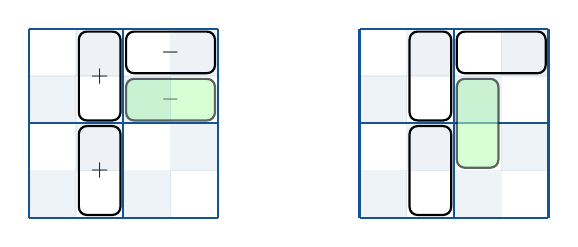
\begin{tikzpicture}[tableau, scale=.6]
    \gridLinesShift{2}{2}{5}
    \verticalDominoShift{1}{2}{+}{5}
    \verticalDominoShift{3}{2}{+}{5}
    \horizontalDominoShift{1}{3}{-}{5}
    \horizontalDominoRSShift{2}{3}{-}{5}
    \fixedSquaresForGridShift{2}{2}{5}
    \gridLinesShift{2}{2}{12}
    \verticalDominoShift{1}{2}{}{12}
    \horizontalDominoShift{1}{3}{}{12}
    \verticalDominoShift{3}{2}{}{12}
    \verticalDominoRSShift{2}{3}{}{12}
    \fixedSquaresForGridShiftAlt{2}{2}{12}
    \end{tikzpicture}
  \end{figure}

  \begin{figure}[H]
    % 1+ 3s 4s 2_5
    \centering
    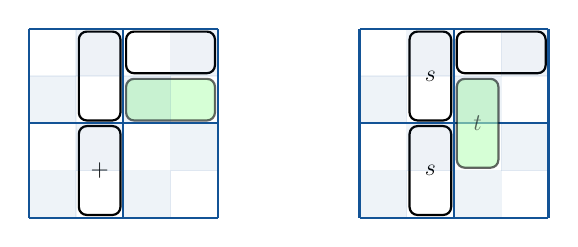
\begin{tikzpicture}[tableau, scale=.6]
    \gridLinesShift{2}{2}{5}
    \verticalDominoShift{1}{2}{}{5}
    \verticalDominoShift{3}{2}{+}{5}
    \horizontalDominoShift{1}{3}{}{5}
    \horizontalDominoRSShift{2}{3}{}{5}
    \fixedSquaresForGridShift{2}{2}{5}
    \gridLinesShift{2}{2}{12}
    \verticalDominoShift{1}{2}{s}{12}
    \horizontalDominoShift{1}{3}{}{12}
    \verticalDominoShift{3}{2}{s}{12}
    \verticalDominoRSShift{2}{3}{t}{12}
    \fixedSquaresForGridShiftAlt{2}{2}{12}
    \end{tikzpicture}
  \end{figure}

  \begin{figure}[H]
    % 1s 2_-4 3_5
    \centering
    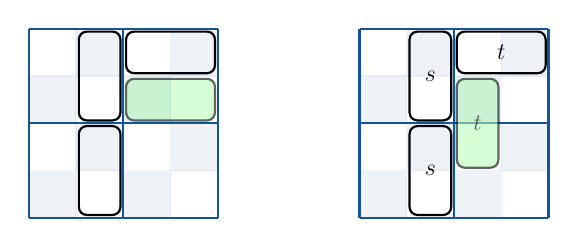
\begin{tikzpicture}[tableau, scale=.6]
    \gridLinesShift{2}{2}{5}
    \verticalDominoShift{1}{2}{}{5}
    \verticalDominoShift{3}{2}{}{5}
    \horizontalDominoShift{1}{3}{}{5}
    \horizontalDominoRSShift{2}{3}{}{5}
    \fixedSquaresForGridShift{2}{2}{5}
    \gridLinesShift{2}{2}{12}
    \verticalDominoShift{1}{2}{s}{12}
    \horizontalDominoShift{1}{3}{t}{12}
    \verticalDominoShift{3}{2}{s}{12}
    \verticalDominoRSShift{2}{3}{t}{12}
    \fixedSquaresForGridShiftAlt{2}{2}{12}
    \end{tikzpicture}
  \end{figure}

  \begin{figure}[H]
    % 1s 2s 4t 3_-5
    \centering
    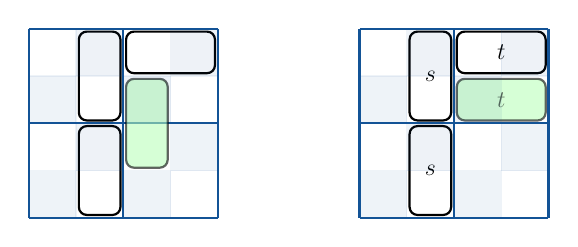
\begin{tikzpicture}[tableau, scale=.6]
    \gridLinesShift{2}{2}{12}
    \verticalDominoShift{1}{2}{}{12}
    \horizontalDominoShift{1}{3}{}{12}
    \verticalDominoShift{3}{2}{}{12}
    \verticalDominoRSShift{2}{3}{}{12}
    \fixedSquaresForGridShiftAlt{2}{2}{12}
    \gridLinesShift{2}{2}{19}
    \verticalDominoShift{1}{2}{s}{19}
    \verticalDominoShift{3}{2}{s}{19}
    \horizontalDominoShift{1}{3}{t}{19}
    \horizontalDominoRSShift{2}{3}{t}{19}
    \fixedSquaresForGridShift{2}{2}{19}
    \end{tikzpicture}
  \end{figure}

  \begin{figure}[H]
    % 1s 3+ 4+ 2_-5
    \centering
    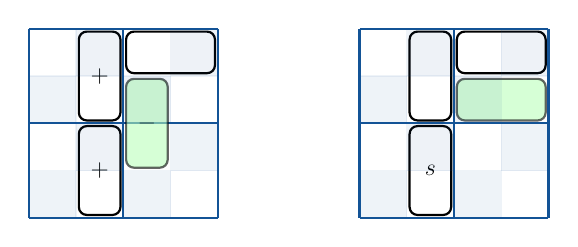
\begin{tikzpicture}[tableau, scale=.6]
    \gridLinesShift{2}{2}{12}
    \verticalDominoShift{1}{2}{+}{12}
    \horizontalDominoShift{1}{3}{}{12}
    \verticalDominoShift{3}{2}{+}{12}
    \verticalDominoRSShift{2}{3}{-}{12}
    \fixedSquaresForGridShiftAlt{2}{2}{12}
    \gridLinesShift{2}{2}{19}
    \verticalDominoShift{1}{2}{}{19}
    \verticalDominoShift{3}{2}{s}{19}
    \horizontalDominoShift{1}{3}{}{19}
    \horizontalDominoRSShift{2}{3}{}{19}
    \fixedSquaresForGridShift{2}{2}{19}
    \end{tikzpicture}
  \end{figure}

  \begin{figure}[H]
    % 1+ 2_4 3_-5
    \centering
    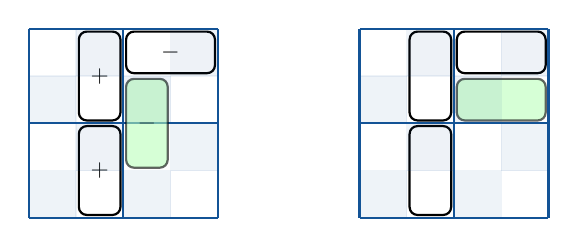
\begin{tikzpicture}[tableau, scale=.6]
    \gridLinesShift{2}{2}{12}
    \verticalDominoShift{1}{2}{+}{12}
    \horizontalDominoShift{1}{3}{-}{12}
    \verticalDominoShift{3}{2}{+}{12}
    \verticalDominoRSShift{2}{3}{-}{12}
    \fixedSquaresForGridShiftAlt{2}{2}{12}
    \gridLinesShift{2}{2}{19}
    \verticalDominoShift{1}{2}{}{19}
    \verticalDominoShift{3}{2}{}{19}
    \horizontalDominoShift{1}{3}{}{19}
    \horizontalDominoRSShift{2}{3}{}{19}
    \fixedSquaresForGridShift{2}{2}{19}
    \end{tikzpicture}
  \end{figure}

  In almost all these configurations, the new top domino is the same or alternating sign to the previous on which it's adjacent to, and we're done now.
  In the fifth case, it isn't.
  So, we have to put that sign into the cycle.
  And then we're done.
\end{document}
